\chapter{\ccplot Manual}\label{chap:ccplot-manual}
As a command-line application, \ccplot is especially convenient for batch
processing. On the other hand, the end user is required to know the names of
command-line options and arguments in order to utilise the program. We provide
an easy-to-follow tutorial on how to use \ccplot in the next section.

\section{Tutorial}
\subsection{Getting started}
In this tutorial we suppose that you have access to a host system running
unix-like operating system such as \program{Linux} with \ccplot
already installed\footnote{To install \ccplot, download the source
distribution of \ccplot from \url{http://www.ccplot.org}, and follow the installation
instructions
included.}, and you
know how to use command-line programs. Moreover, it should be a host with at
least \SI{1}{GB} of physical memory, \SI{4}{GB} is recommended. Start by simply running the
program with the \texttt{-V} (print version) option:

\begin{alltt}
\$ ccplot -V
ccplot 1.31

Third-party libraries:
matplotlib 0.98.1
basemap 0.99.4

Copyright 2009, 2010 Peter Kuma.
This software is provided under the terms of a 2-clause BSD licence.
\end{alltt}

\noindent If no errors were reported, the required third-party libraries are
present on the
host system, and you can continue with the tutorial.

\subsection{Getting Information}
For brevity, we will assume
that the shell variable \texttt{\$HDF} is set to a directory where the HDF files
reside.
Prepare a CloudSat 2B-GEOPROF product such as
\textit{2006224184641\_01550\_CS\_2B-GEOPROF\_GRANULE\_P\_R03\_E01.hdf} and
enter:


\begin{alltt}
\$ ccplot -i
\$HDF\textit{/2006224184641_01550_CS_2B-GEOPROF_GRANULE_P_R03_E01.hdf}
Type: CloudSat
Time: 2006-08-12 18:46:41, 2006-08-12 20:25:34
Height: -4874, 24865
nray: 37088
nbin: 125
Longitude: 104.171097, 79.441208
Latitude: 0.009954, -0.036672
\end{alltt}

\noindent The \texttt{-i} switch instructs \ccplot to print summary information
about the file.

\subsection{Plotting Atmosphere Profiles}
To plot the first 1000 rays of the Radar Reflectivity Factor
data set and save it as \textit{cloudsat1.pdf}, enter:

\begin{alltt}
\$ ccplot -o \textit{cloudsat1.pdf} -x 0..1000 cloudsat-reflec
\$HDF/\texttt{2006224184641\_01550\_CS\_2B-GEOPROF\_GRANULE\_P\_R03\_E01.hdf}
\end{alltt}

\begin{figure}[t]
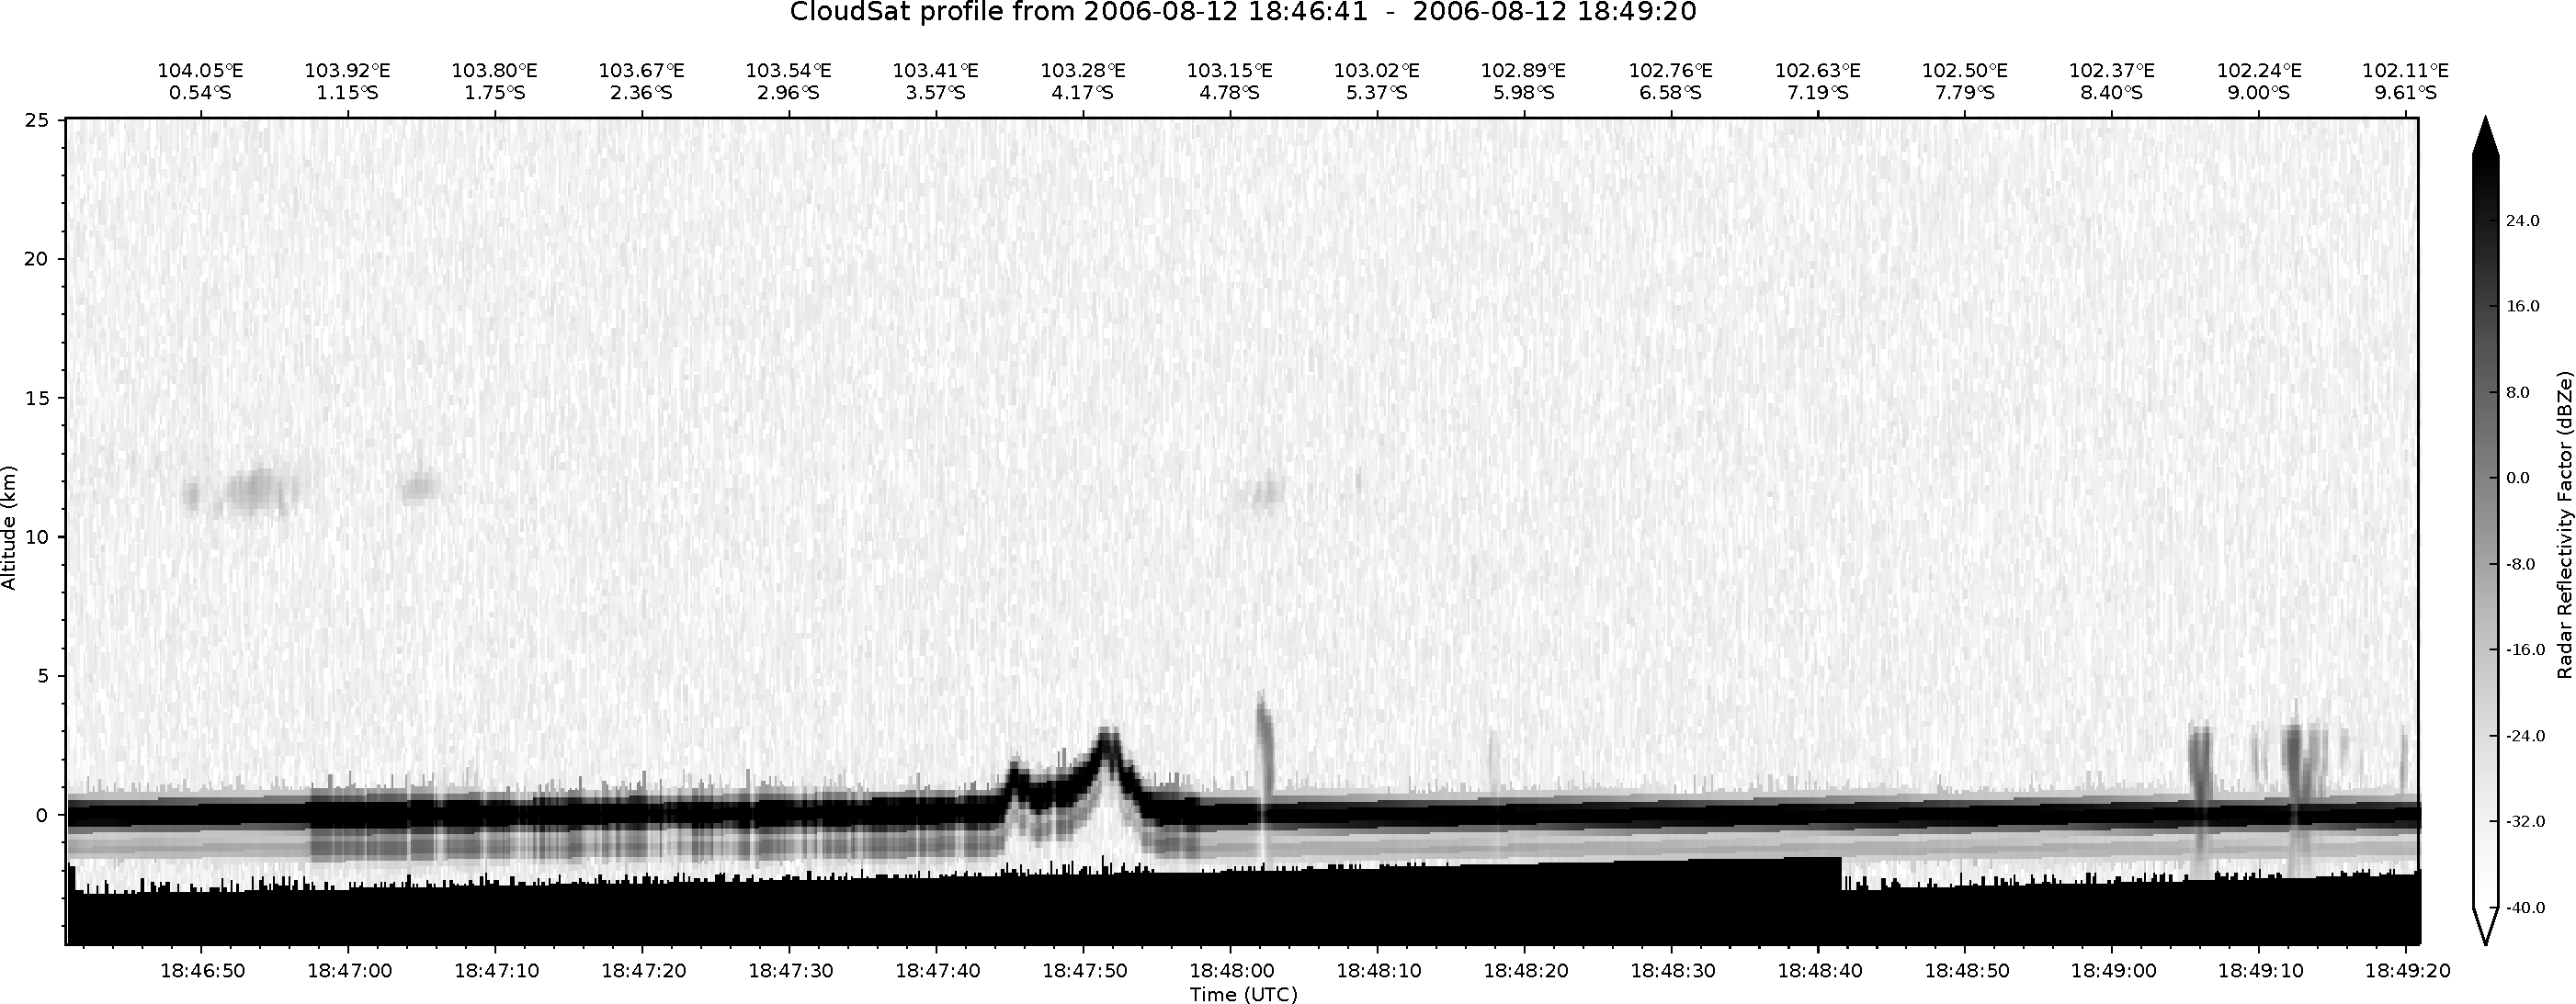
\includegraphics[width=\textwidth]{images/cloudsat1.pdf}
\caption[cloudsat1.pdf]{\textbf{cloudsat1.pdf}}
\label{fig:cloudsat1}
\end{figure}

\begin{figure}[t]
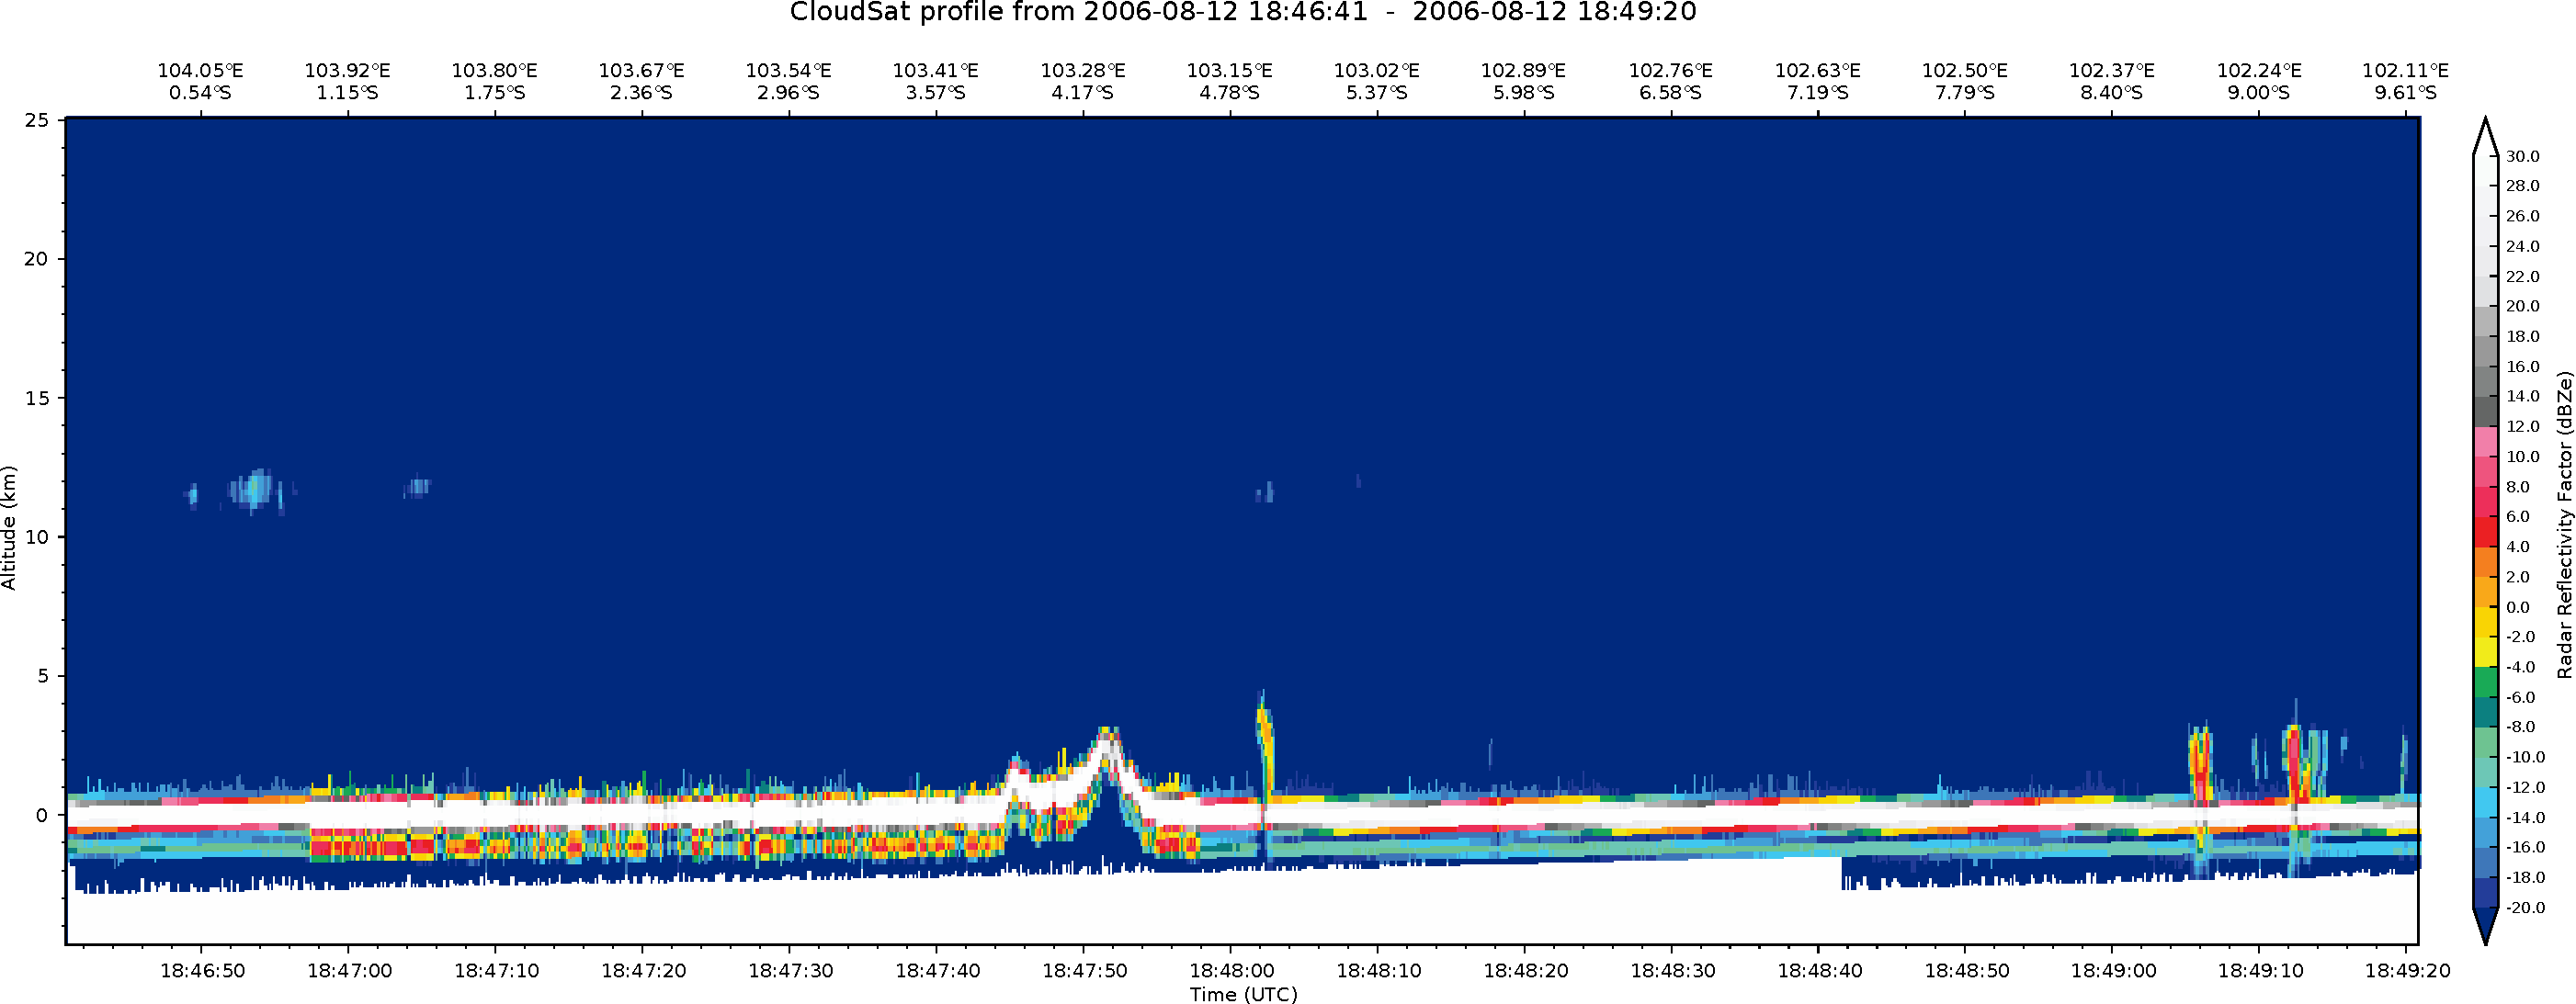
\includegraphics[width=\textwidth]{images/cloudsat2.pdf}
\caption[cloudsat2.pdf]{\textbf{cloudsat2.pdf}}
\label{fig:cloudsat2}
\end{figure}

\noindent You should get an image similar to that in
Fig.\,\ref{fig:cloudsat1}.  The
\texttt{-x} option tells \ccplot what extent to plot, and \texttt{ccplot-reflec}
chooses the CloudSat Radar Reflectivity Factor as the input. The \texttt{-o}
option selects the output file. The result may not seem very impressive, but we
have not yet selected any colormap. Therefore, \ccplot will use the default
colormap, which is a black-and-white gradient spanning the entire valid range of
the selected data set. Fortunately, \ccplot comes with a set of colormaps that
you can use without making your own. These are stored in
\texttt{\$PREFIX}\textit{/share/ccplot/cmap}, where \texttt{\$PREFIX} is the
installation prefix, usually \textit{/usr} or \textit{/usr/local}. The one
suitable for \texttt{cloudsat-reflec} is \textit{cloudsat-reflectivity.cmap}.
Let us use it in the next example (Fig.\,\ref{fig:cloudsat2}):

\begin{figure}[t]
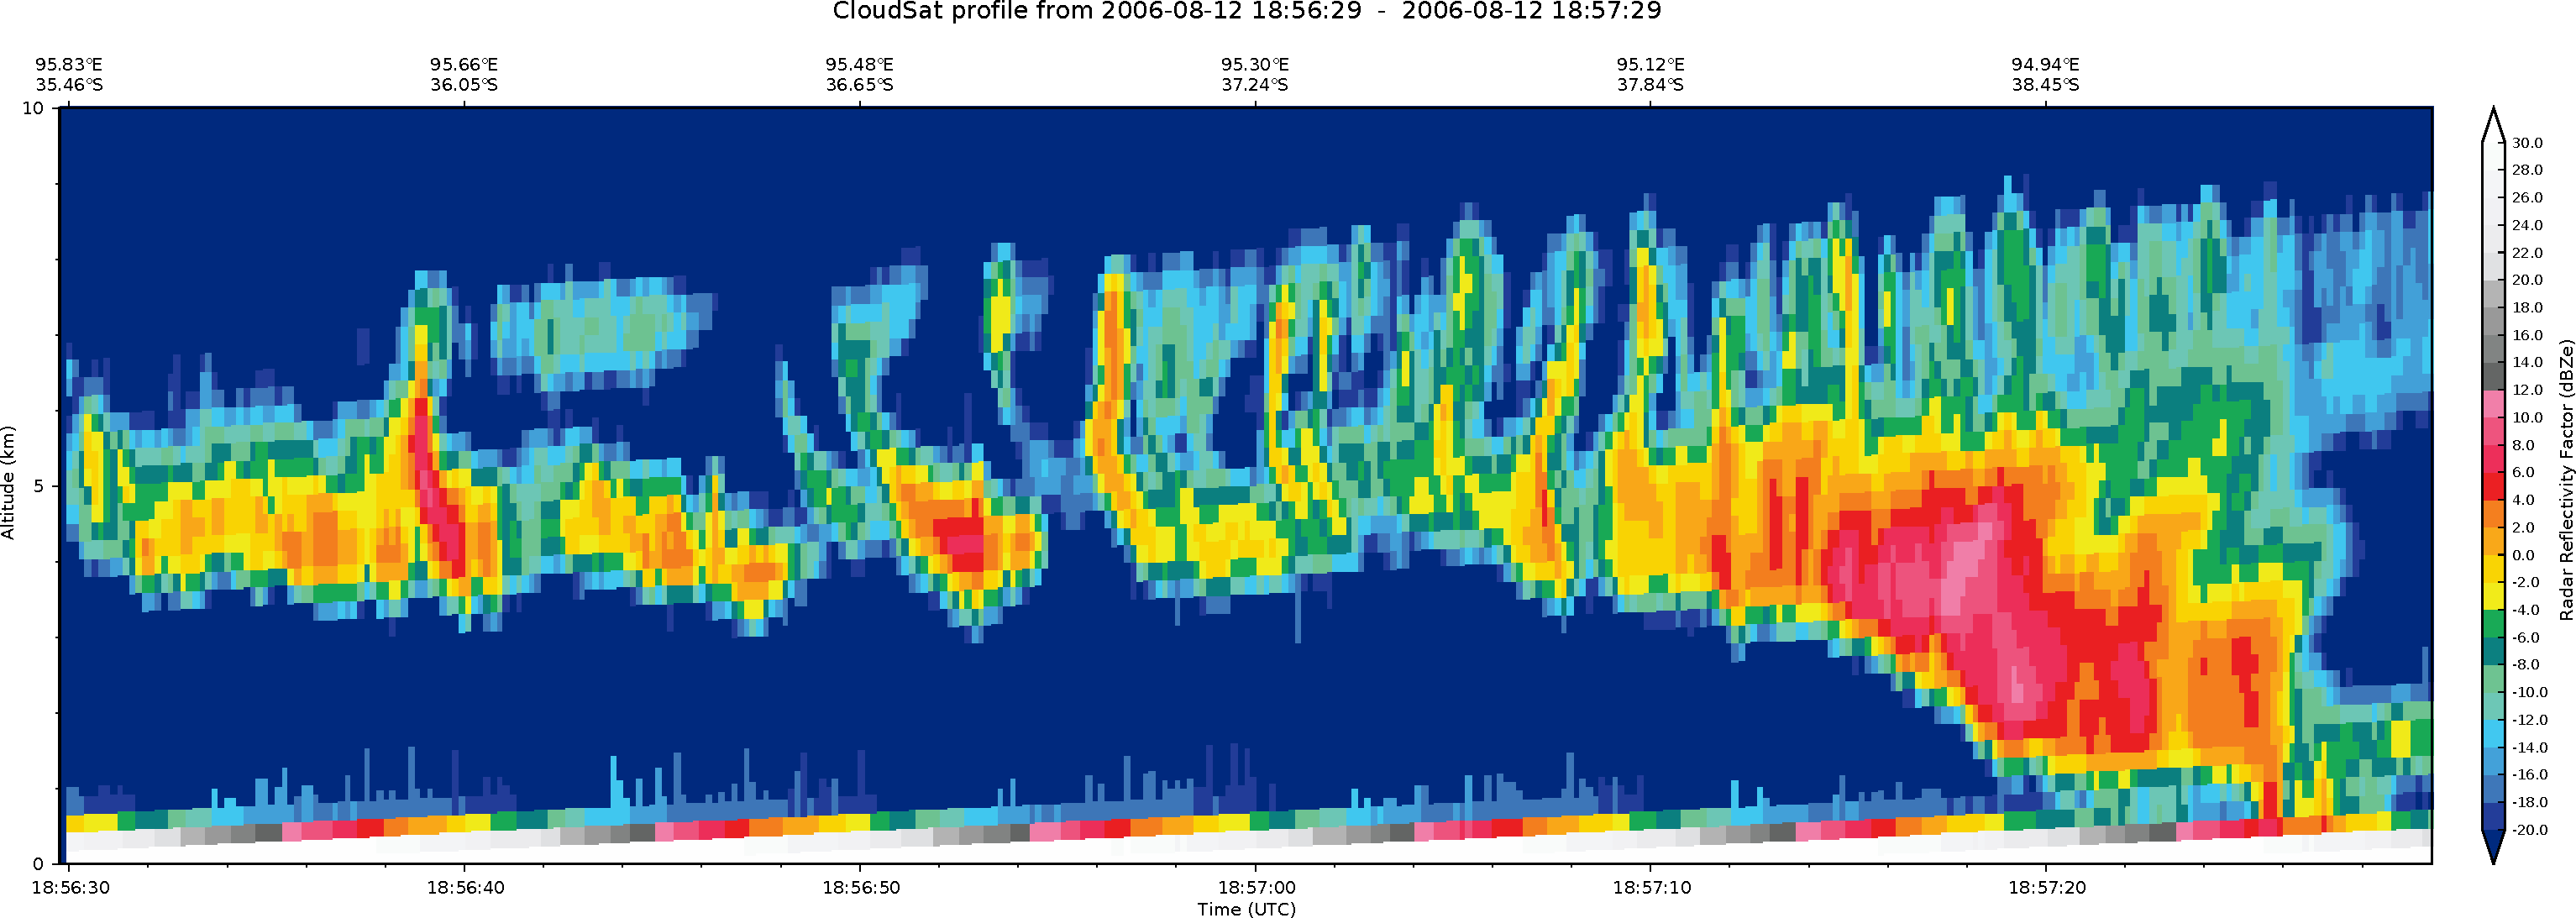
\includegraphics[width=\textwidth]{images/cloudsat3.pdf}
\caption[cloudsat3.pdf]{\textbf{cloudsat3.pdf}}
\label{fig:cloudsat3}
\end{figure}

\begin{figure}[t]
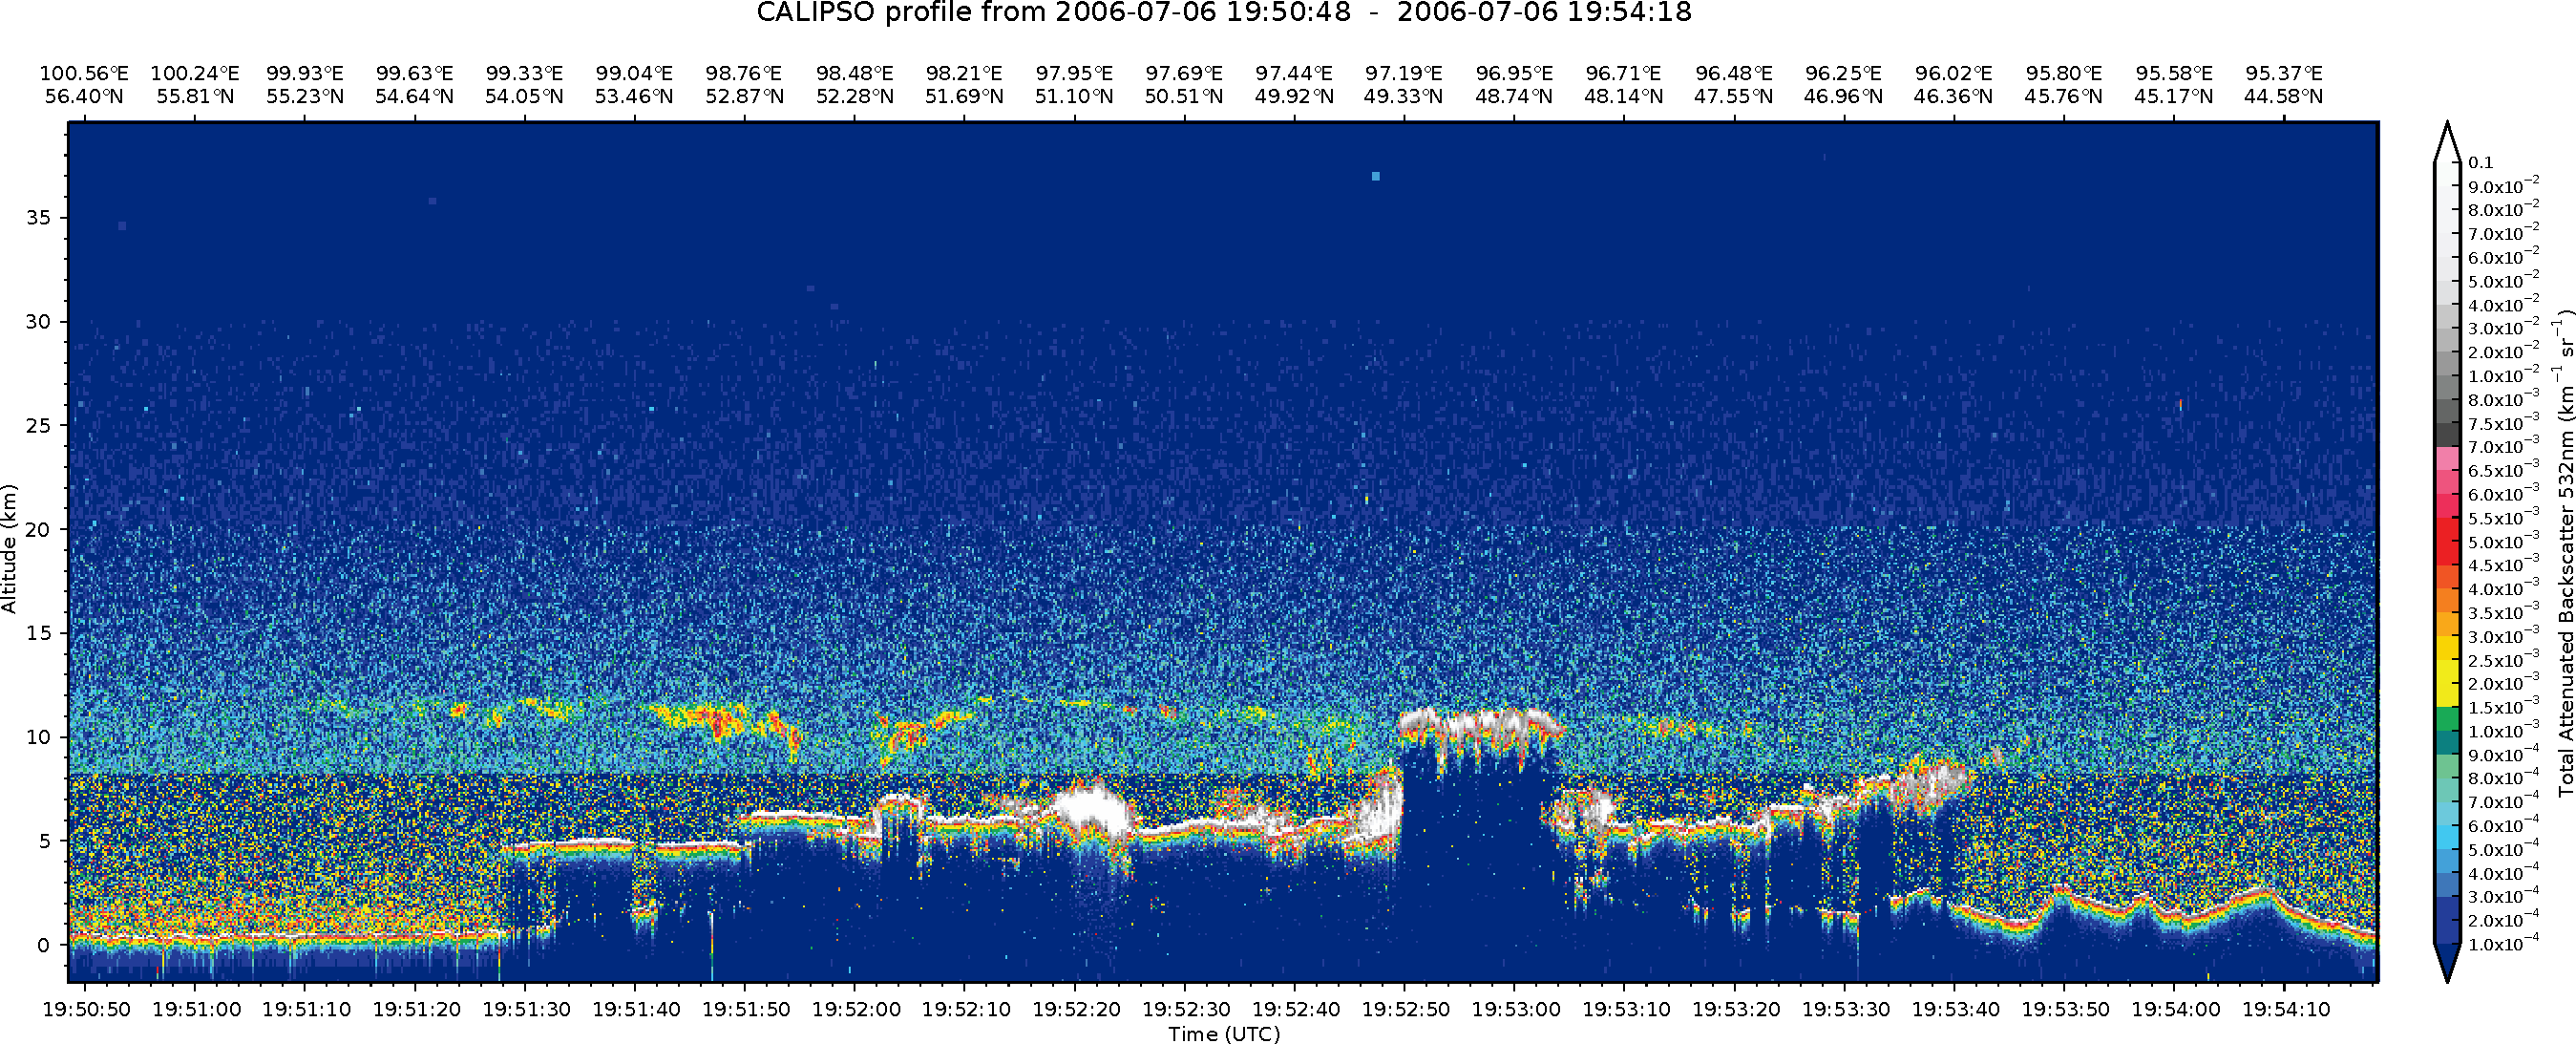
\includegraphics[width=\textwidth]{images/calipso1.pdf}
\caption[calipso1.pdf]{\textbf{calipso1.pdf}}
\label{fig:calipso1}
\end{figure}

\begin{alltt}
\$ ccplot -o \textit{cloudsat2.pdf} -x 0..1000
-c \textit{/usr/share/ccplot/cmap/cloudsat-reflectivity.cmap} cloudsat-reflec
\$HDF/\textit{2006224184641_01550_CS_2B-GEOPROF_GRANULE_P_R03_E01.hdf}
\end{alltt}

\noindent This demonstrates the use of the \texttt{-c} (colormap) option.
Fig.\,\ref{fig:colormaps} contains a summary of colormaps supplied with \ccplot,
and Section\,\ref{sec:colormaps}\, will
guide you through the process of crating your own colormap.


Suppose you know that there is an interesting feature between 18:56:30 and
18:57:30 UTC, which spans 0--\SI{10}{km} vertically. You can use the \texttt{-x}
option with an absolute time, and select the vertical extent in meters with the
\texttt{-y} option (Fig.\,\ref{fig:cloudsat3}):

\begin{alltt}
\$ ccplot -o \textit{cloudsat3.pdf} -x 18:56:30..18:57:30 -y 0..10000
-c \textit{/usr/share/ccplot/cmap/cloudsat-reflectivity.cmap}
cloudsat-reflec
\$HDF/\textit{2006224184641_01550_CS_2B-GEOPROF_GRANULE_P_R03_E01.hdf}
\end{alltt}

\subsection{CALIPSO}

\noindent Plotting CALIPSO products is almost identical to plotting CloudSat
products. The only difference is that CALIPSO products are in higher resolution
than those of CloudSat. Therefore, a 1000-ray plot of CALIPSO backscatter would
likely be too short.

\begin{figure}[t]
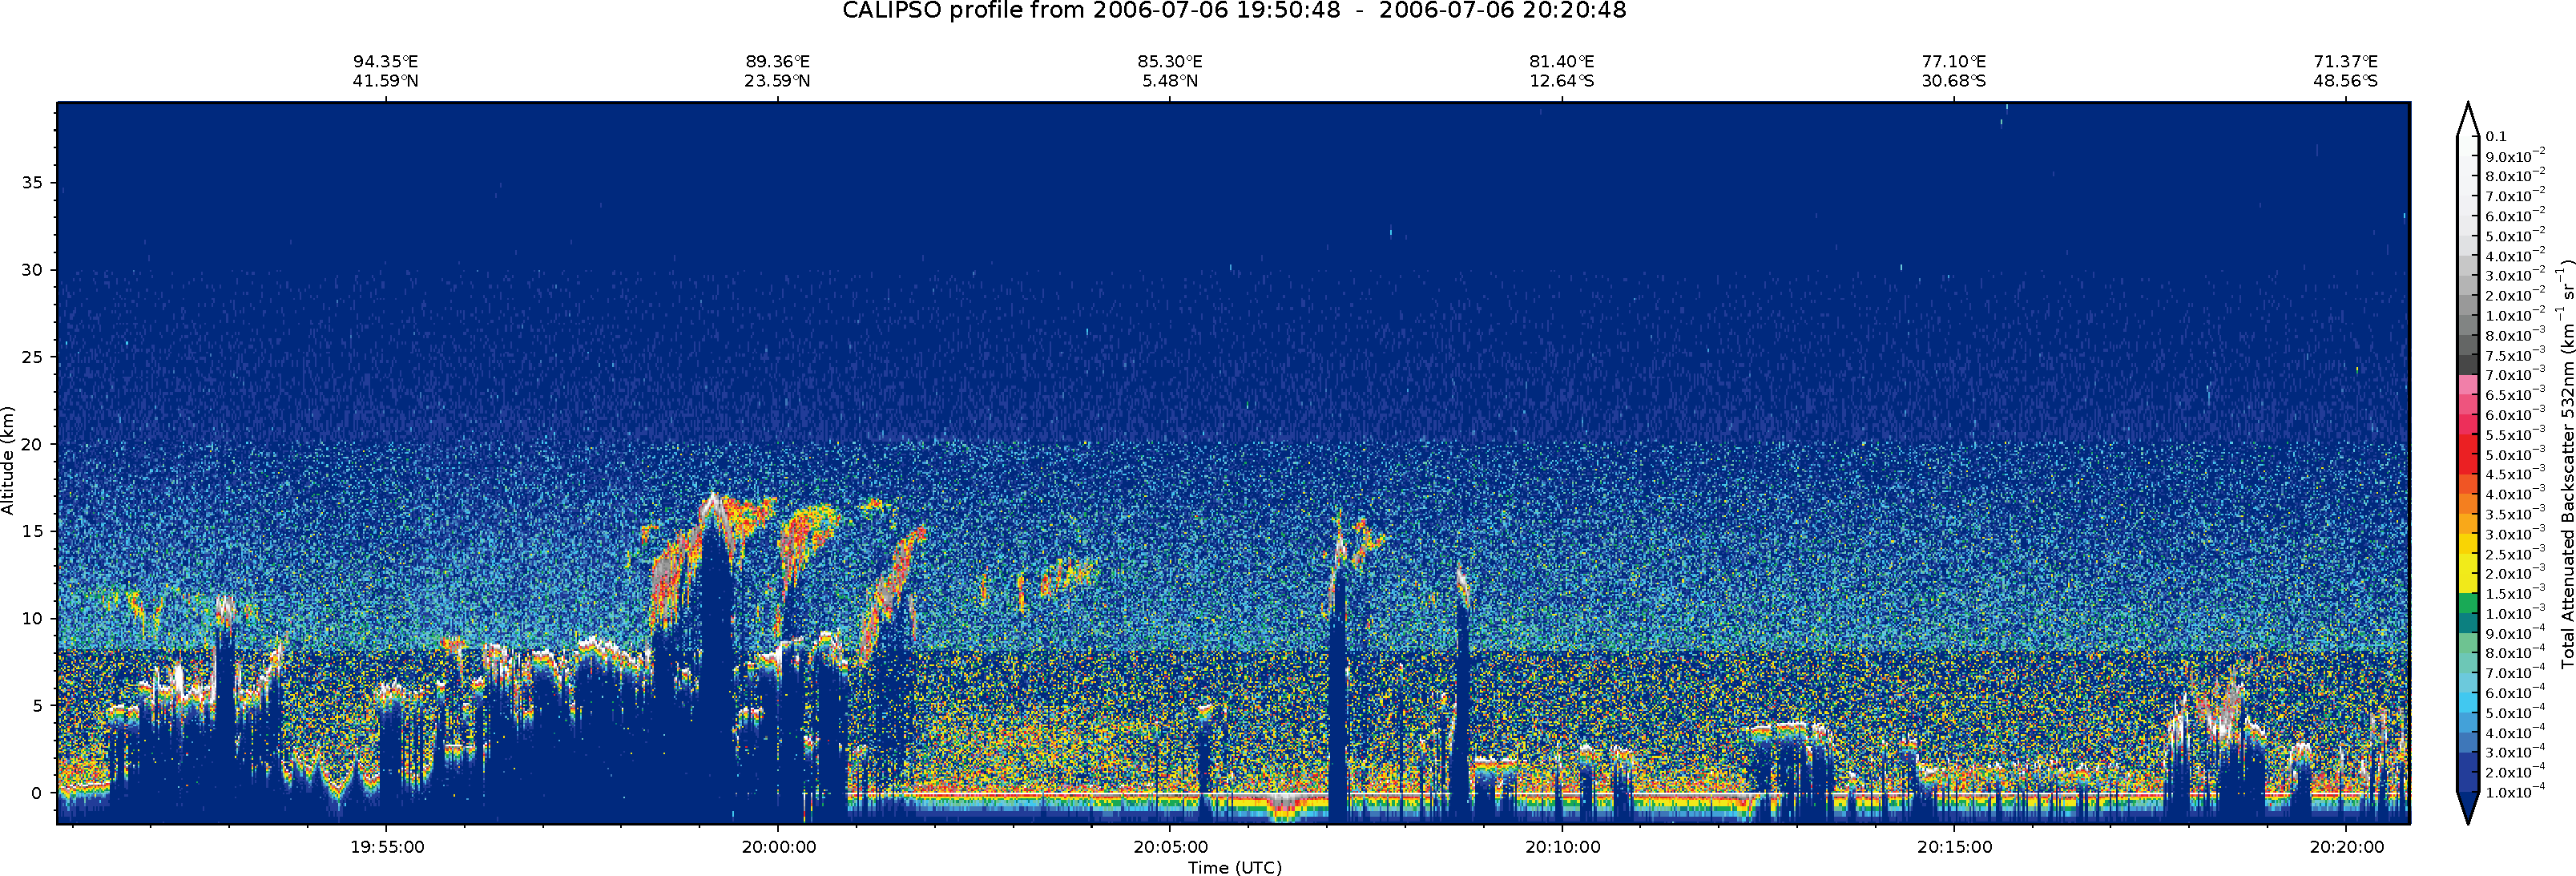
\includegraphics[width=\textwidth]{images/calipso2.pdf}
\caption[calipso2.pdf]{\textbf{calipso2.pdf}}
\label{fig:calipso2}
\end{figure}

\begin{figure}[t]
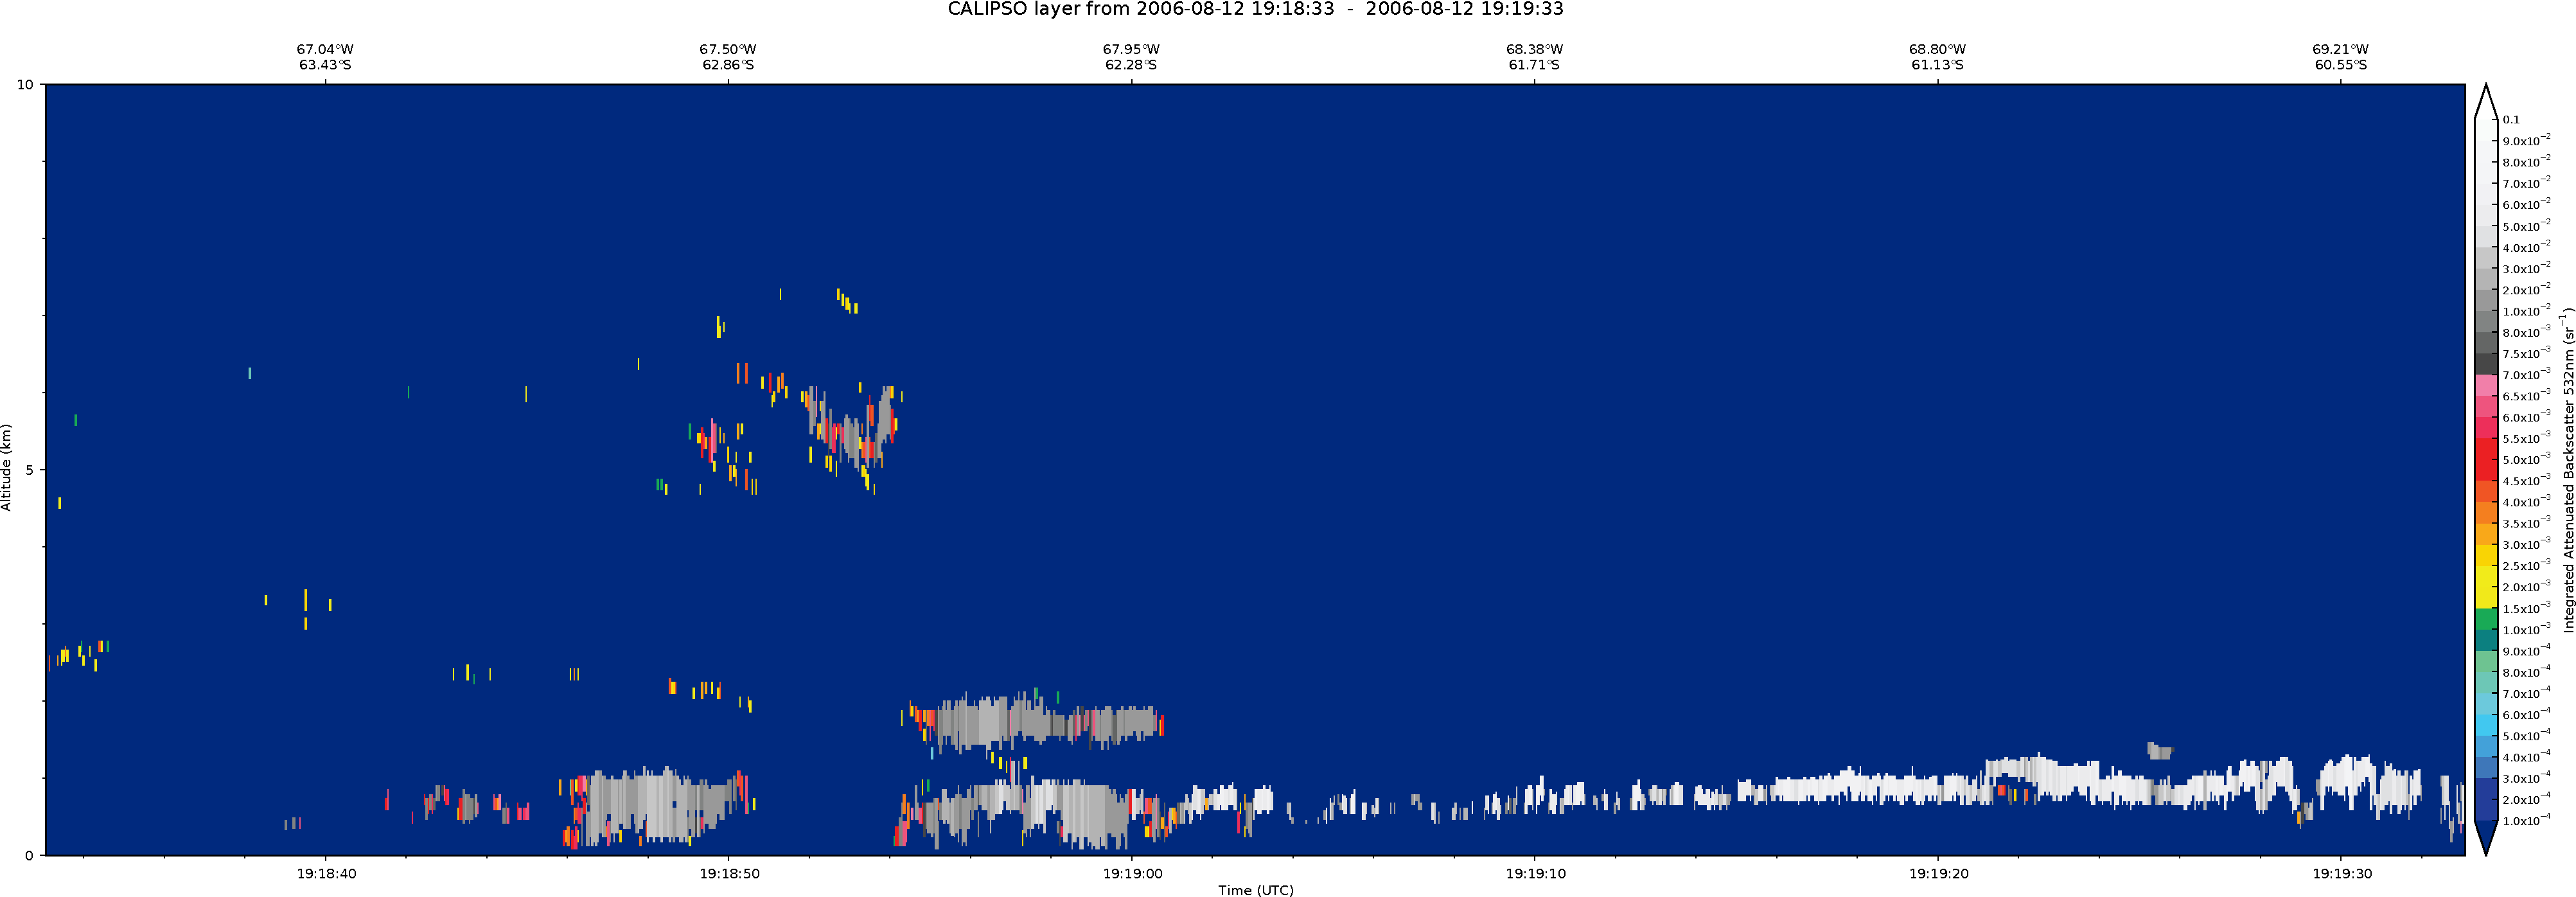
\includegraphics[width=\textwidth]{images/calipso3.pdf}
\caption[calipso3.pdf]{\textbf{calipso3.pdf}}
\label{fig:calipso3}
\end{figure}

We will now focus on some of the advanced features. Prepare one CALIPSO
L1B Profile product, and one CALIPSO L2 Layer product. Let us start with the L1B
product, and use the \texttt{-d} option to change the DPI of the resulting
image. The default DPI is 300 pixels per inch. This time, we will use the
\texttt{-x} option with a relative time in the format \texttt{(+|-)[HH]:MM:SS}.
The preceding plus sign means `\textit{relative to the beginning}', whereas the minus
sign means `\textit{relative to the end}'.

\begin{alltt}
\$ ccplot -o \textit{calipso1.pdf} -d 100 -x +0:00..+3:30
-c \textit{/usr/share/ccplot/cmap/calipso-backscatter.cmap} calipso532
\$HDF/\textit{CAL_LID_L1-Prov-V2-01.2006-07-06T19-50-51ZN.hdf}
\end{alltt}


\noindent This command plots the first three-and-a-half minutes of
Total Attenuated Backscatter 532nm in 100 pixels per inch. The result is in
Fig.\,\ref{fig:calipso1}.
\ccplot in its default configuration does not plot profiles in 1:1 aspect ratio,
as the plots would appear squashed in the vertical direction. We chose the
aspect ratio 14 as the default.
For example, if you wanted to plot 30 minutes of a profile in one plot
without it being too long, you could increase the aspect ratio to 1:10000
(Fig.\,\ref{fig:calipso2}):

\begin{alltt}
\$ ccplot -o \textit{calipso2.pdf} -a 10000 -x +0:00..+30:00
-c \textit{/usr/share/ccplot/cmap/calipso-backscatter.cmap} calipso532
\$HDF/\textit{CAL_LID_L1-Prov-V2-01.2006-07-06T19-50-51ZN.hdf}
\end{alltt}

\noindent Last but not least, \ccplot allow you to change the size of the plot
in inches.
You can change the height of the data part of the plot --- the axes, but also the
padding (space on the margins of the canvas), and spacing between the axes and
the color bar. Supplementary options like these are covered by the \texttt{-z}
option, which takes a list of comma-separated \texttt{name=value} pairs as its
argument. The default value of the \textit{plotheight} option is \SI{6}{in}. Suppose you
want to change the plot height to \SI{8}{in}, the padding to \SI{1.2}{in}, and
the axes-color bar spacing to
\SI{0.1}{in}. We will try this new setting on a layer product
(Fig.\,\ref{fig:calipso3}):

\begin{alltt}
\$ ccplot -o \textit{calipso3.pdf} -x +3:00..+4:00 -y 0..10000
-z plotheight=8,padding=1.2,cbspacing=0.1 -c
\textit{/usr/share/ccplot/cmap/calipso-backscatter.cmap} calipso532-layer
\$HDF/\textit{CAL_LID_L2_333mCLay-Prov-V2-01.2006-08-12T19-15-34ZD.hdf}
\end{alltt}


\begin{figure}[p]
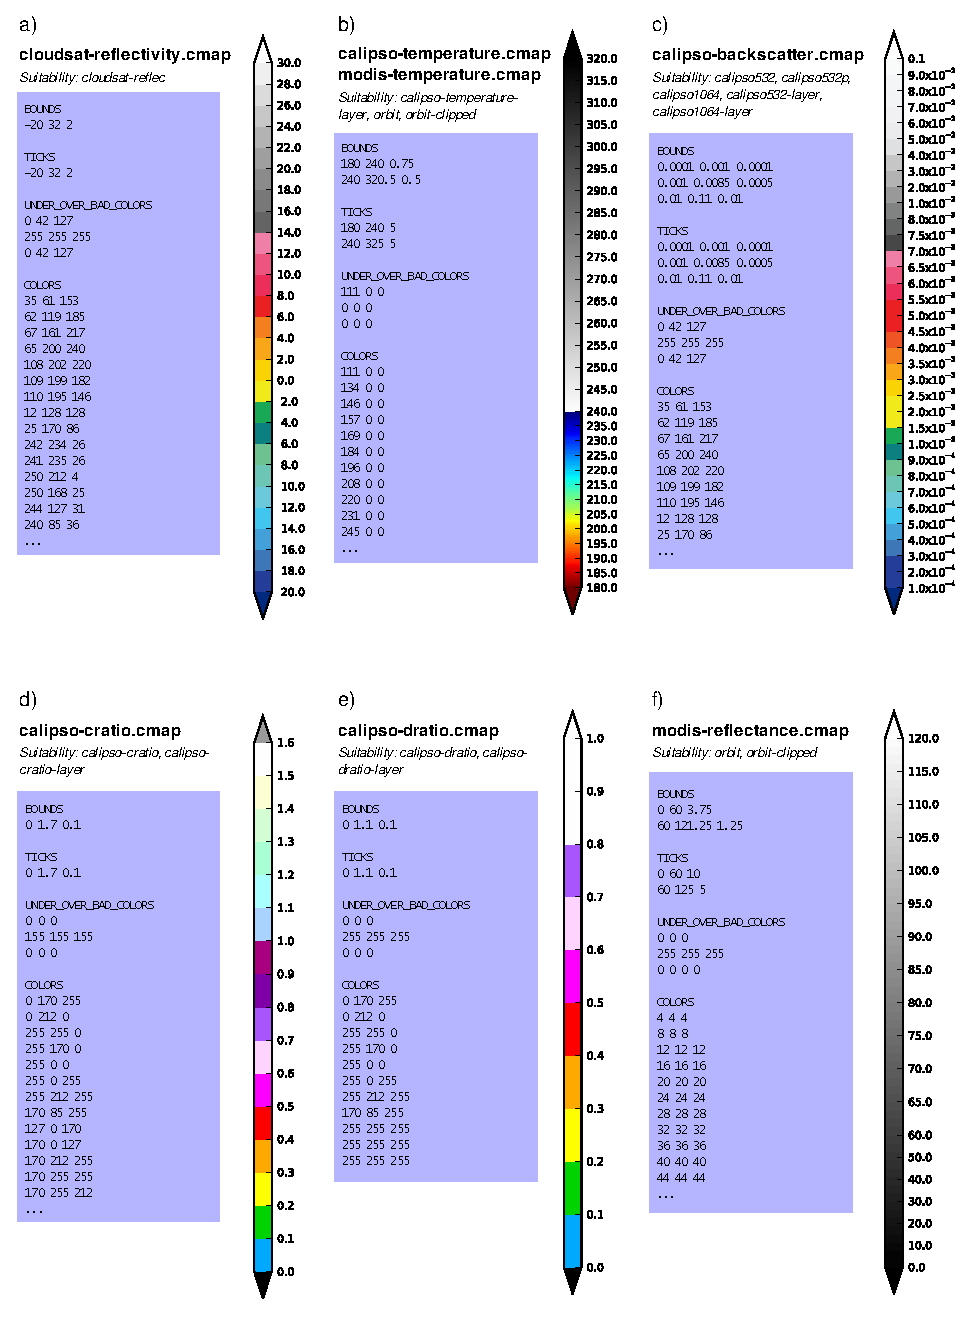
\includegraphics[width=\textwidth]{images/colormaps.pdf}
\caption[Colormaps supplied with ccplot]{\textbf{Colormaps supplied with ccplot.}}
\label{fig:colormaps}
\end{figure}

\section{How to Create Your Own Colormap}\label{sec:colormaps}

If none of the colormaps supplied with \ccplot suits your needs, you can create
your own. \ccplot colormaps are stored in simple ASCII text files. Some example
colormaps are in Fig.\,\ref{fig:colormaps}. You can start by creating a copy of
one of these
files, and replacing the various sections of the file. As explained the previous
section, colormaps can typically be found in \textit{/usr/share/ccplot/cmap}
or \textit{/usr/local/share/ccplot/cmap}. A colormap file divided into four sections
- \texttt{BOUNDS}, \texttt{TICKS}, \texttt{UNDER\_OVER\_BAD\_COLORS} and
\texttt{COLORS}. These can appear in an arbitrary order in the file. The start
of a section
is denoted by a section header (section name in capital letters). Blank lines
are
ignored.

\begin{description}

\item[\textbf{\texttt{BOUNDS}}] This section describes the boundaries. Values
that lie between two boundaries are mapped to the same colour. Boundaries are
specified by ranges in the form \texttt{start stop step}, i.e. three floating
point numbers separated by white space. For example, \texttt{0 10 2} would
produce boundaries at 0, 2, 4, 6, 8. Notice that \texttt{stop} is not included
in the range. \texttt{BOUNDS} section can contain multiple lines of one range
per line. Ranges should be specified in an increasing order.

\item[\textbf{\texttt{TICKS}}] This section specifies where ticks on the
colorbar should be placed. The format is the same as the format of
\texttt{BOUNDS}.

\item[\textbf{\texttt{UNDER\_OVER\_BAD\_COLORS}}] This section contains three
colours. The first one (\textit{under}) is used for values that lie below the lowest
boundary. The second one (\textit{over}) is used for values that lie above the
highest boundary. The third one (\textit{bad}) is used for points where there is no valid
data. Colours are specified by three (optionally four) numbers separated by
white space. These are the RGB or RGBA (Red, Green, Blue, Alpha) components encoded in an 8-bit-per-channel
base-10 format (i.e. values between 0 and 255, incl.).

\item[\textbf{\texttt{COLORS}}] This section contains the colours which data
values
lying between respective boundaries are mapped onto. The first colour
following the section header is the one that lies between the first two
boundaries, and so on. Colours in this section are in the same format as colours
in the \texttt{UNDER\_OVER\_BAD\_COLORS} section described above.

\end{description}

\noindent When creating custom colormaps, you should take into consideration
that the performance of the current implementation of \ccplot depends
significantly on the number of color entries in the colormap. This is an
inherent problem of the plotting library \program{matplotlib}, but we may be
able to
alleviate it in one of the future versions of \ccplot.

